\documentclass[10pt]{article}

\usepackage[T1]{fontenc}
\usepackage[utf8]{inputenc}
%\usepackage{beton}
%\usepackage{ccfonts}
%\usepackage{concrete}
\usepackage{concmath}
\usepackage{eulervm}
\usepackage{amsmath,amsthm,amssymb}
\usepackage{mathtools}
\usepackage{multicol}
\usepackage{marginnote}
\usepackage{pgfplots}
\usepackage{float}
\usepackage{hyperref}
\usepackage{bbm}
\usepackage{booktabs}
\usepackage{xcolor-solarized}
\usepackage{xcolor}
\pgfplotsset{compat=1.5}

\usepackage{listings}
\usepackage{xcolor}
\definecolor{codegreen}{rgb}{0,0.6,0}
\definecolor{codegray}{rgb}{0.5,0.5,0.5}
\definecolor{codepurple}{rgb}{0.58,0,0.82}
\definecolor{backcolour}{rgb}{0.95,0.95,0.92}
\lstdefinestyle{mystyle}{
    backgroundcolor=\color{backcolour},   
    commentstyle=\color{codegreen},
    keywordstyle=\color{magenta},
    numberstyle=\tiny\color{codegray},
    stringstyle=\color{codepurple},
    basicstyle=\ttfamily\footnotesize,
    breakatwhitespace=false,         
    breaklines=true,                 
    captionpos=b,                    
    keepspaces=true,                 
    numbers=left,                    
    numbersep=5pt,                  
    showspaces=false,                
    showstringspaces=false,
    showtabs=false,                  
    tabsize=2
}

\lstset{language=Python, style=mystyle}

\usepackage{mathtools}

\usepackage{wasysym}
\usepackage[margin=1.5in]{geometry} 
\usepackage{enumerate}
\index{\usepackage}\usepackage{multicol}

\newcommand{\N}{\mathbf{N}}
\newcommand{\Z}{\mathbb{Z}}

\newcommand{\R}{\mathbf{R}}
\newcommand{\C}{\mathbf{C}}
\newcommand{\Pbb}{\mathbb{P}}
\newcommand{\Fcal}{\mathcal{F}}
\newcommand{\Lcal}{\mathcal{L}}
\newcommand{\Acal}{\mathcal{A}}
\newcommand{\Ecal}{\mathcal{E}}
\newcommand{\Ebb}{\mathbb{E}}
\newcommand{\Qbb}{\mathbb{Q}}


\renewcommand{\mathbf}{\mathbold}

\newenvironment{theorem}[2][Theorem]{\begin{trivlist}
  \item[\hskip \labelsep {\bfseries #1}\hskip \labelsep {\bfseries #2.}]}{\end{trivlist}}
\newenvironment{lemma}[2][Lemma]{\begin{trivlist}
  \item[\hskip \labelsep {\bfseries #1}\hskip \labelsep {\bfseries #2.}]}{\end{trivlist}}
\newenvironment{exercise}[2][Exercise]{\begin{trivlist}
  \item[\hskip \labelsep {\bfseries #1}\hskip \labelsep {\bfseries #2.}]}{\end{trivlist}}
\newenvironment{reflection}[2][Reflection]{\begin{trivlist}
  \item[\hskip \labelsep {\bfseries #1}\hskip \labelsep {\bfseries #2.}]}{\end{trivlist}}
\newenvironment{proposition}[2][Proposition]{\begin{trivlist}
  \item[\hskip \labelsep {\bfseries #1}\hskip \labelsep {\bfseries #2.}]}{\end{trivlist}}
\newenvironment{corollary}[2][Corollary]{\begin{trivlist}
  \item[\hskip \labelsep {\bfseries #1}\hskip \labelsep {\bfseries #2.}]}{\end{trivlist}}

\newenvironment{definition}[2][Definition]{\begin{trivlist}
  \item[\hskip \labelsep {\bfseries #1}\hskip \labelsep {\bfseries #2.}]}{\end{trivlist}}

\definecolor{solar}{rgb}{0.9960, 0.9960, 0.9647}

\begin{document}
  \pagecolor{solar}
	
  \renewcommand{\qedsymbol}{\smiley}
	\title{Investments Class \\ Problem set 7}
	\author{Daniel Grosu, William Martin, Denis Steffen}
		
\maketitle

\begin{exercise}{1}(Portfolio choice with liabilities)
  \begin{itemize}
    \item The investor can invest in the risky assets with expected returns $\mu$ and in the riskless asset with return $R_0$. So the expected return of the portfolio is: $$ \Ebb[R_p] = w'\mu + R_0w_0 = w'\mu + R_0(1-w'\mathbbm{1})$$
    So the optimization problem becomes: 
    $$ \max_w \left(w'\mu + R_0(1-w'\mathbbm{1}) -\frac{a}{2}w'\Sigma w\right)$$ and there is no constraint, so the Lagrangien function equals this expression. 
    \\
    We differentiate with respect to $w$ and get:
    $$ \frac{\partial \mathcal{L}}{\partial w} = \mu - R_0\mathbbm{1} - a \Sigma w $$ and the optimal $w$ is: 
    $$ w = \frac{1}{a}\Sigma^{-1}(\mu- R_0\mathbbm{1})$$
    $$ w_0 = 1 - \frac{1}{a}(\mu- R_0\mathbbm{1})'\Sigma^{-1}\mathbbm{1}$$

    We can rewrite the weights in risky assets as: 
    $$ w = \frac{B-R_0A}{a}w_{tan} \quad \text{with } w_{tan} = \frac{\Sigma^{-1}(\mu-R_0\mathbbm{1})}{B-R_0A}$$
    
    Thus, the investor can invest in two funds, the tangency portfolio that is independent of the risk-aversion and only consists of risky assets, with coefficient $ \frac{B-R_0A}{a}$ and in the riskfree asset with coefficient $w_0$. 

    If the risk-aversion tends to infinity, we can see that $w_0 \rightarrow 1$ and $w \rightarrow \mathbf{0} $, so she invests only in the riskfree asset. This is consistent, because she does not want to take any risk. 
    \item Now, the investor has access to a liability $L$. So the function to be optimized becomes: 
    $$ \Ebb[R_p - L] - \frac{a}{2}Var(R_p-L) = w'\mu +R_0(1-w'\mathbbm{1}) - \mu_L - \frac{a}{2}(w'\Sigma w + \sigma_L - 2\Sigma_L'w)$$ because $\Ebb[L] = \mu_L$ and  $$Var(R_p - L) = Var(R_p) + Var(L) - 2Cov(R_p,L)  = w'\Sigma w + \sigma_L - 2\Sigma_L'w$$

    Again, there is no constraint, so we can differentiate the Lagrangien: 
    $$ \frac{\partial \mathcal{L}}{\partial w} = \mu -R_0\mathbbm{1} - a\Sigma w + a\Sigma_L$$ and the optimal weights equal:
    $$ w = \frac{1}{a}\left(\Sigma^{-1}(\mu-R_0\mathbbm{1})\right) + \Sigma^{-1}\Sigma_L $$
    $$ w_0 = 1 - \left(\frac{1}{a}(\mu-R_0\mathbbm{1})'\Sigma^{-1}\mathbbm{1} + \Sigma_L'\Sigma^{-1}\mathbbm{1}\right)$$

    \item Now, if we set $w_L = \Sigma^{-1}\Sigma_L$, we end up with a three-fund separation because the investor invests in $w_{tan}$ the tangency portfolio (only in risky assets), in the riskless asset and in $w_L$. 
    $$ w = \frac{B-R_0A}{a}w_{tan} + w_L \quad \text{and } w_0 = 1 - w'\mathbbm{1}$$

    If the risk aversion becomes infinitely large, than $w = w_L$ and $w_0 = 1 - w_L$. This can be understood as follows: 
    \\
    As the investor is infinitely risk averse, so she does not want to hold risky securities, she only wants to invest in the riskless asset (as in the previous case). However, she has to pay back her liability $L$ and therefore she can only invest $1 - w_L$ in the risk-free asset. The liability is considered as a risky investment and so $w = w_L$ because she will pay back the liability (we can say equivalently, that she invests $w_L$). 
  \end{itemize}
\end{exercise}


\begin{exercise}{2}

  The results of the MCAP-quantile portfolios computed based on the MCAP values
  on date December 31, 2019 and on the lagged MCAP values are presented in
  \autoref{tbl:december2019} and \autoref{tbl:lagged}. The excess returns
  plotted against beta are shown in \autoref{fig:december2019} and
  \autoref{fig:lagged}; and the alphas of the both types of portfolios are plotted in
\autoref{fig:alphas}.

  (b) The equally weighted excess returns of the quantile portfolios based on the
  MCAP on date December 31, 2019, seem to be mostly constant except for the
  portfolios with the lowest and highest market capitalizations. The weighted
  returns seem to increase with the market capitalizations. The CAPM cannot
  explain this behavior. The CAPM posits that the excess returns depend only on
  the betas of the portfolios, not on the market capitalizations. We can see,
  however, that the market capitalization of the stocks can be used as a proxy
  for their betas since portfolios of ``small stocks'' have higher beta and
  those of ``big stocks'' have a lower beta. However, even when the excess
  returns are controlled for the market risk, abnormal returns exist which remain
  unexplained (alphas in \autoref{tbl:december2019}). This is due to the fact
  that the portfolios are computed based on the last date of the sample.
  Moreover, the weighted excess returns behave contrarily to the CAPM: it seems
  that the market premium is negative. This anomaly is not surprising since
  these portfolios do not take into account the time variation of the market
  capitalization of stocks.
  \begin{figure}[n]
    \centering
    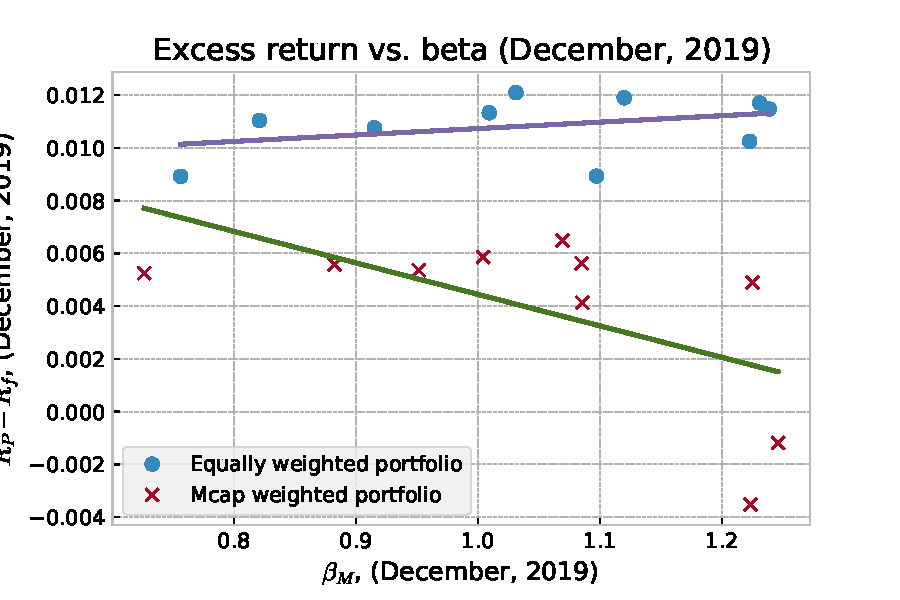
\includegraphics[width=0.7\linewidth]{december2019.pdf}
    \caption{The Excess returns of the MCAP-quantiles portfolios computed at
      December 31, 2019 against the betas of the portfolios between January 1,
      2000 and December 31, 2019}
    \label{fig:december2019}
  \end{figure}
  \begin{figure}[H]
    \centering
    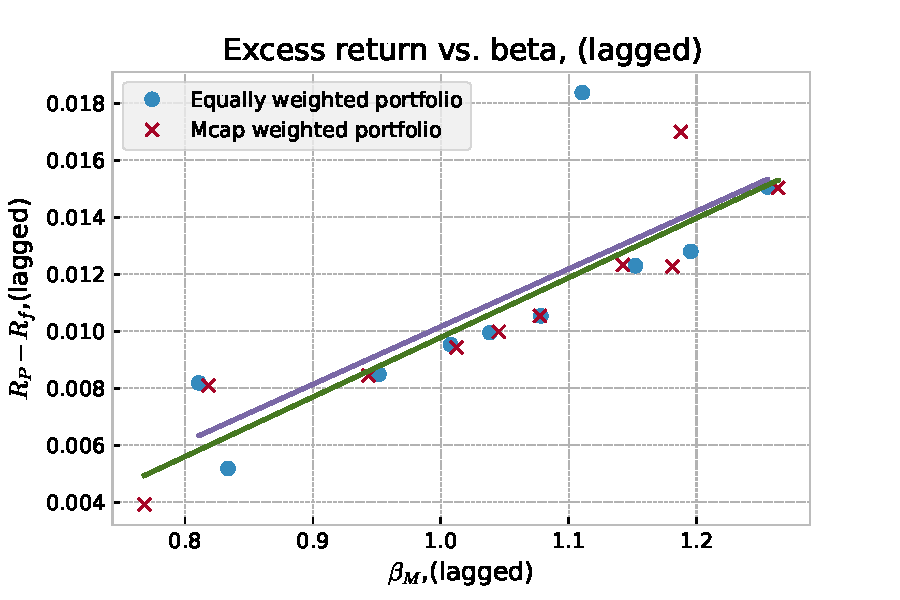
\includegraphics[width=0.7\linewidth]{lagged.pdf}
    \caption{The Excess returns of the MCAP-quantiles portfolios computed on
      lagged MCAP values against the betas of the portfolios between January 1,
      2000 and December 31, 2019}
    \label{fig:lagged}
  \end{figure}
  \begin{figure}[H]
    \centering
    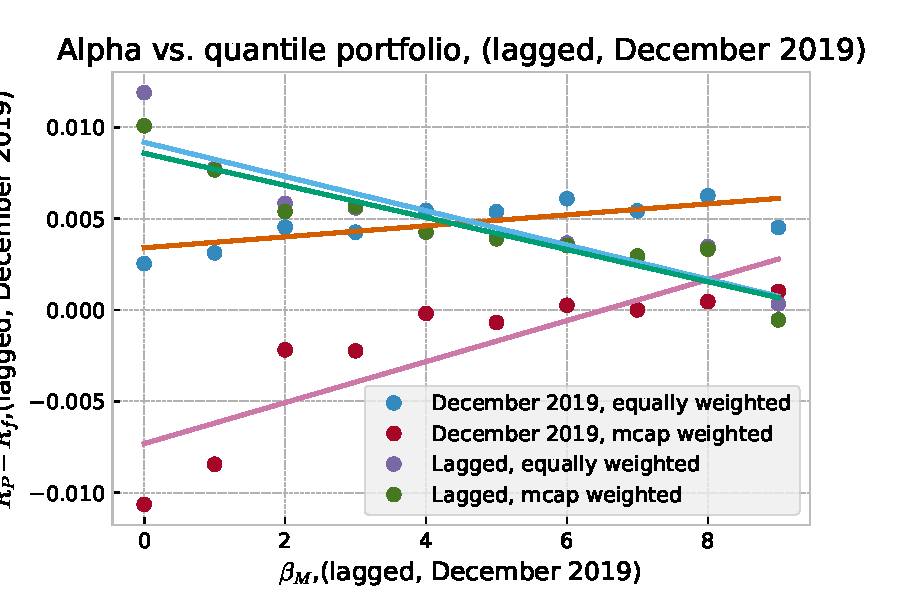
\includegraphics[width=0.7\linewidth]{alphas.pdf}
    \caption{Equally and Weighted alphas for the MCAP-quantiles portfolios
      computed on date December 31, 2019 and on the lagged MCAP values.}
    \label{fig:alphas}
  \end{figure}


  (d) The inverse proportional relation between the excess returns and the MCAP
  is clearly visible in the Lagged construction of the portfolios: small stocks
  have an average of $1.8\%$ monthly returns but the big stocks an average of
  only $0.5\%$. Judging based on the alphas which according to the CAPM should
  be zero, the evidence for the validity of the CAPM depends tremendously on the
  type of stocks considered. In the \autoref{tbl:lagged} are shown the
  decreasing alphas from small stocks to big stocks.


\begin{table}
\centering
\begin{tabular}{|c|cccccc|}
\toprule
Portfolio &  $R^{e}_{P} - R_m$&  $R^{w}_{P} - R_m$ &    $\beta_e$ &   $\alpha_e$ &    $\beta_w$ &  $\alpha_w$ \\
\midrule
0.0           &  0.008928 & -0.003519 &  1.097198 &  0.002537 &  1.223557 & -0.010647 \\
1.0           &  0.010247 & -0.001188 &  1.222773 &  0.003124 &  1.246237 & -0.008448 \\
2.0           &  0.011706 &  0.004136 &  1.230999 &  0.004535 &  1.085347 & -0.002187 \\
3.0           &  0.011472 &  0.004897 &  1.238775 &  0.004256 &  1.224935 & -0.002239 \\
4.0           &  0.011330 &  0.005356 &  1.009298 &  0.005450 &  0.951568 & -0.000187 \\
5.0           &  0.011898 &  0.005630 &  1.119895 &  0.005375 &  1.084977 & -0.000690 \\
6.0           &  0.012096 &  0.006487 &  1.031097 &  0.006089 &  1.069309 &  0.000258 \\
7.0           &  0.010760 &  0.005853 &  0.915078 &  0.005429 &  1.004329 &  0.000002 \\
8.0           &  0.011037 &  0.005593 &  0.821006 &  0.006254 &  0.882363 &  0.000453 \\
9.0           &  0.008921 &  0.005244 &  0.756289 &  0.004515 &  0.726412 &  0.001013 \\
\bottomrule
\end{tabular}
\caption{The excess returns, betas and alphas of the MCAP-quantiles portfolios
  computed based on the Mcap at December 31, 2019.}
\label{tbl:december2019}
\end{table}


\begin{table}
\centering
\begin{tabular}{|c|cccccc|}
\toprule
Portfolio &  $R^{e}_{P} - R_m$&  $R^{w}_{P} - R_m$ &    $\beta_e$ &   $\alpha_e$ &    $\beta_w$ &  $\alpha_w$ \\
\midrule
0.0             &  0.018372 &  0.017005 &  1.110667 &  0.011902 &  1.187857 &  0.010085 \\
1.0             &  0.015059 &  0.015031 &  1.255630 &  0.007744 &  1.263970 &  0.007668 \\
2.0             &  0.012802 &  0.012271 &  1.195533 &  0.005838 &  1.181005 &  0.005391 \\
3.0             &  0.012300 &  0.012330 &  1.152240 &  0.005587 &  1.142339 &  0.005675 \\
4.0             &  0.010540 &  0.010551 &  1.078297 &  0.004258 &  1.077576 &  0.004273 \\
5.0             &  0.009951 &  0.009990 &  1.038437 &  0.003902 &  1.045504 &  0.003900 \\
6.0             &  0.009529 &  0.009428 &  1.007763 &  0.003659 &  1.012575 &  0.003529 \\
7.0             &  0.008497 &  0.008451 &  0.951659 &  0.002953 &  0.943707 &  0.002953 \\
8.0             &  0.008189 &  0.008099 &  0.810882 &  0.003465 &  0.818240 &  0.003333 \\
9.0             &  0.005191 &  0.003929 &  0.833616 &  0.000335 &  0.768089 & -0.000546 \\
\bottomrule
\end{tabular}
\caption{The excess returns, betas and alphas (equally and MCAP-weighted) of the MCAP-quantiles portfolios
  computed based on the lagged Mcap.}
\label{tbl:lagged}
\end{table}

\end{exercise}
  
\end{document}



\appendix
